\documentclass[12pt,a4paper]{report}
\usepackage[utf8]{inputenc}
\usepackage[inner=3.5cm,outer=2.5cm,bottom=3cm,top=2.5cm,pdftex]{geometry}
\usepackage{setspace}
\usepackage{graphicx}
\usepackage{rotating}
\usepackage[page]{appendix}
\usepackage{float}
\usepackage[font=small,labelfont=bf]{caption}
\usepackage{subfigure}
\usepackage{titlesec}
\usepackage[hidelinks]{hyperref}
\usepackage{listings}
\usepackage{textcomp}
\usepackage{fancyhdr}
\usepackage{multirow}
\usepackage{verbatim}	%makes it possible to comment out a section of text by using \begin{comment}...\end{comment}
\usepackage[table,xcdraw]{xcolor}
\usepackage{pifont}
\usepackage{mathptmx}
\usepackage{wrapfig}
\usepackage{ragged2e}
\usepackage[nottoc,notlot,notlof]{tocbibind}
\usepackage[norsk]{babel}
\usepackage[final]{pdfpages}

\definecolor{rockwoolcolor}{RGB}{155,0,0}

% Style chapter headings for preface and toc.
\setlength{\headheight}{15pt}
\titlespacing*{\chapter}{0pt}{0pt}{4ex}
\titleformat{\chapter}[display]
 {\bfseries\Large}
 {}
 {0pt}
 {\color{rockwoolcolor}\titlerule[2.0pt]\vspace{2ex}\filright\color{black}}
 [\color{rockwoolcolor}\vspace{2ex}{\titlerule[2.0pt]}]


\setstretch{1.25}
\begin{document}
\begin{titlepage}

\newcommand{\HRule}{\color{rockwoolcolor}\rule{\linewidth}{0.75mm}\color{black}} % Defines a new command for the horizontal lines, change thickness here

\center % Center everything on the page
 
%----------------------------------------------------------------------------------------
%	HEADING SECTIONS
%----------------------------------------------------------------------------------------
\ \\[1.5cm]
\textsc{\LARGE BI Handelshøyskolen}\\[1.5cm] % Name of your university/college
\textsc{\Large BTH 95031 Økonomistyring og investeringsanalyse}\\[2.5cm] % Major heading such as course name


%----------------------------------------------------------------------------------------
%	TITLE SECTION
%----------------------------------------------------------------------------------------

\HRule \\[0.4cm]
{ \huge \bfseries Investeringsanalyse for \\[0.5cm] ROCKWOOL International}\\[0.4cm] % Title of your document
\HRule \\[2.5cm]
 
%----------------------------------------------------------------------------------------
%	DATE & PLACE SECTION
%----------------------------------------------------------------------------------------

{\large \textbf{Innleveringsdato:}\\  \today}\\[1cm] % Date, change the \today to a set date if you want to be precise
{\large \textbf{Studiested:}\\  BI Nydalen}\\[3cm] % Date, change the \today to a set date if you want to be precise
 
%----------------------------------------------------------------------------------------

\textit{Denne oppgaven er gjennomført som en del av studiet ved Handelshøyskolen BI. Dette innebærer
ikke at Handelshøyskolen BI går god for de metoder som er anvendt, de resultater som er
fremkommet, eller de konklusjoner som er trukket.}
\vfill % Fill the rest of the page with whitespace

\end{titlepage}
{\RaggedRight
\pagestyle{fancy}

% empty default settings for fancy layout
\fancyhf{}

% table mark commands
\newcommand{\cmark}{\textcolor{green!80!black}{\ding{51}}}
\newcommand{\xmark}{\textcolor{red}{\ding{55}}}
\newcommand{\plusmark}{\textcolor{green!80!black}{\textbf{+}}}
\newcommand{\minusmark}{\textcolor{red}{\textbf{-}}}

% chapter, section, header and footer layout
\renewcommand{\sectionmark}[1]{\markright{\thesection ~ \ #1}}
\renewcommand{\chaptermark}[1]{\markboth{ #1}{}}
\renewcommand{\headrulewidth}{0.5pt}
\renewcommand{\footrulewidth}{0.5pt}

%head setting
%\fancyhead[L]{\textcolor{black} {\rightmark}}
\fancyfoot[C]{\textcolor{black} {\thepage}}

% Redefine the plain page style - used when the page is a chapter
\fancypagestyle{plain}{%
  \fancyhf{}%
  \renewcommand{\headrulewidth}{0pt}% Line at the header invisible
  \renewcommand{\footrulewidth}{0.5pt}% Line at the footer visible
  \fancyfoot[C]{\textcolor{black} {\thepage}}
}

% Avoid hyphenating
\tolerance=10
\emergencystretch=\maxdimen
\hyphenpenalty=10000
\hbadness=10000

\pagenumbering{roman}
\chapter*{Forord}



\chapter*{Sammendrag}
I desember 2018 besluttet ROCKWOOL International å investere i en ny elektrisk smelteovn på fabrikken i Moss. Konsernet produserer isolasjonsprodukter som utvinnes av vulkansk stein, og er verdens ledende leverandør av produkter og løsninger basert på steinull. Formålet med oppgaven er å utføre en investeringsanalyse på vegne av selskapet for å undersøke om prosjektet er lønnsomt. 

\indent \newline
For å vurdere lønnsomheten av prosjektet benytter vi oss av netto nåverdimetoden. Beregningen er basert på en differansekontantstrøm som er utarbeidet ved å sammenligne nåværende smelteteknologi med den nye elektriske smelteovnen. Kontantstrømmene neddiskonteres med relevant avkastningskrav justert for valutarisiko og business risk. Avkastningskravet er estimert gjennom beregning av selskapets egenkapitalbeta som brukes til å beregne egenkapitalkrav og selskapets totalkapitalkrav.

\indent \newline
I oppgaven drøfter vi ulike makroforhold som legges til grunn for fremtidig utvikling i isolasjonsbransjen. Den viktigste faktoren er det globale fokuset mot en grønnere fremtid. Analysen viser til flere usikkerhetsmomenter som er vanskelig å forutse hvordan vil utvikle seg i fremtiden. Sensitivitetsanalyser er derfor benyttet for å belyse hvordan endringer i forutsetningene vil påvirke netto nåverdi. I tillegg har vi utført en \textit{best-} og \textit{worst} case analyse for å gjøre ledelsen i selskapet bevisst på utfallsrommet investeringen befinner seg i.

\indent \newline
Differansekontantstrømmen  viser til en positiv netto nåverdi på 588,500 millioner kroner og gir støtte til å konkludere med at investeringen er lønnsom. I tillegg vil prosjektet styrke selskapets merkevare og gi bedre forutsetninger til å imøtekomme endringen i markedsutviklingen.


\setcounter{tocdepth}{2}
\tableofcontents
\addtocontents{toc}{~\hfill\textbf{Side}\par}
\listoffigures
\listoftables

% ----------- CHAPTERS ----------------

% Parts
\cleardoublepage
% Style chapter headings.
\titleformat{\chapter}[display]
 {\bfseries\Large}
 {}
 {0pt}
 {\color{rockwoolcolor}\titlerule[2.0pt]\vspace{2ex}\filright\color{black} \thechapter . }
 [\color{rockwoolcolor}\vspace{2ex}{\titlerule[2.0pt]}]
\pagenumbering{arabic}
\setcounter{page}{1}
\chapter{Innledning}
\section{Formål}
I denne oppgaven skal vi gjennomføre en investeringsanalyse av AS ROCKWOOL sin beslutning om å investere i en ny elektriske smelteovn. Formålet er å se hvorvidt dette er et lønnsomt prosjekt fra eiernes perspektiv ved tidspunktet for beslutningen. Vi vil gjøre leseren oppmerksom på at oppgaven vil analysere investeringen på bakgrunn av AS ROCKWOOL som et selvstendig selskap? (få frem at vi ikke legger vekt på at bedriften er en del av et konsern, evt finner vi ut av det senere, kanskje det går an å inkludere konsernet i oppgaven?)

\section{Problemstilling}
Problemstillingen vi ønsker å besvare er utarbeidet i samarbeid med AS ROCKWOOL, og lyder som følger:

\indent \newline
\textit{\textbf{Var investeringen av elektrisk smelteovn lønnsom på beslutningstidspunktet?}}

\indent \newline
Lønnsomhetsvurderingen vil baseres på en flerperiodisk nåverdianalyse med et formål om å maksimere eiernes interesser. I dette tilfellet vil investeringen ikke kun vurderes ut i fra et finansielt perspektiv, men også fra ROCKWOOL-konsernets eiere, som ønsker å implementere en mer miljøvennlig profil. Vurderingen vil gjennomføres på følgende grunnlag:

\begin{itemize}
\item Vurdere investeringen isolert sett.
\item Nåverdianalyse av virksomhetens fremtidige kontantstrømmer ved beslutning om å investere i ny produksjonsteknologi.
\item Nåverdianalyse av virksomhetens fremtidige kontantstrømmer ved beslutning om å ikke investere i ny. produksjonsteknologi (fortsette som før).
\item Nåverdianalyse av virksomhetens fremtidige kontantstrømmer ved beslutning om å investere i alternativt “grønt” produksjonsutstyr (BAT-løsning/brun energi).
\end{itemize}

\indent \newline
I tillegg vil vi gjennom scenario(scenarie?)-analyse skissere tre forskjellige fremtider for investeringen (best, basis og worst), for å gjøre ledelsen mest mulig forberedt på fremtidige beslutninger relatert til virksomhetens strategi. (kanskje legge til noe om støtte fra Enova også?) kan være at dette punktet skal smelles inn et annet sted også!

\chapter{ROCKWOOL International og byggisolasjonsbransjen}
Kapittelet vil gi en kort presentasjon av konsernet og datterselskapet AS ROCKWOOL. Videre vil det redegjøres for nåsituasjonen til Rockwool, og hvilke utfordringer virksomheten står overfor i dag.

\section{Om selskapet}
ROCKWOOL International er verdens største steinullprodusent med over 11.000 ansatte fordelt på salgskontorer og fabrikker i 39 land. Virksomheten baseres på utvinning av vulkansk stein for å produsere produkter, systemer og løsninger innenfor byggisolasjon. Selskapet hadde i 2018 salgsinntekter på 26,149 milliarder kroner og et årsresultat på 2,064 milliarder kroner \cite{annualReport}.

\subsection{AS ROCKWOOL}
AS ROCKWOOL er et heleid norsk datterselskap av ROCKWOOL international. Virksomhetens visjon er \textit{“AS ROCKWOOL skal være ledende leverandør av isolasjon, der positivt bidrag til et bedre miljø og brannsikring skal være førende”}. Datterselskapet består av 240 ansatte fordelt på to fabrikker og et salgskontor. Disse er lokalisert i henholdsvis Moss, Trondheim og Oslo. I 2018 hadde de salgsinntekter på 919 millioner kroner og leverte et årsresultat på litt over 86 millioner kroner \cite{osloRegnskap}.

\indent \newline
Produksjonsprosessen foregår ved at vulkansk stein og koks blir tilsatt i den varme enden av maskinen og deretter utsatt for enormt høye temperaturer i en smelteovn. Videre blir det tilsatt bindemiddel hvor den glødende massen blir omgjort til ullfibre før massen spinnes til steinull.

\begin{figure}[H]
\centering
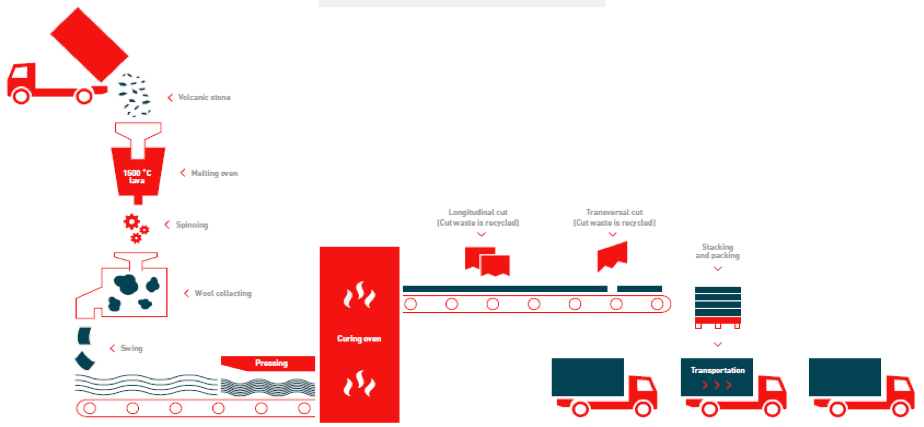
\includegraphics [scale=0.95]{bilder/produksjonsprosess.png}
\caption{Produksjonsprosess}
\label{fig:produksjonsprosess}
\end{figure}

\section{Historie}
I 1937 ble den første Rockwool-fabrikken etablert i Danmark. Få år senere utvidet konsernet med fabrikker i Larvik, Trondheim og Moss. Siden oppstarten i Norge har Rockwool basert virksomheten på utvinning av vulkansk stein, hvor produksjonsprosessen har forandret seg lite. Imidlertid investerte de nærmere en halv milliard kroner i nytt produksjonsutstyr på fabrikken i Moss i 2002, med et formål om å automatisere produksjonen. Dette har ført til mer enn en fordobling av produksjonskapasiteten. I løpet av de siste årene har de innført en lean-metode som de kaller for Ropex, med et ønske om å effektivisere virksomheten gjennom hele verdikjeden \cite{dagsavisen}.

\indent \newline
I 2016 vedtok Rockwool-konsernet å forplikte seg til FNs bærekraftsmål, hvorav 6 av 10 er implementert som interne konsernmål. Målene representerer forbedringer innenfor sikkerhet og helse, vannforbruk, energieffektivitet, avfallsresirkulering, og reduksjon i avfall og CO2-utslipp i produksjonsprosessen. Ett av målene er å redusere CO2-utslippet med 10\% innen 2022 og 20\% innen 2030.

\begin{figure}[H]
\centering
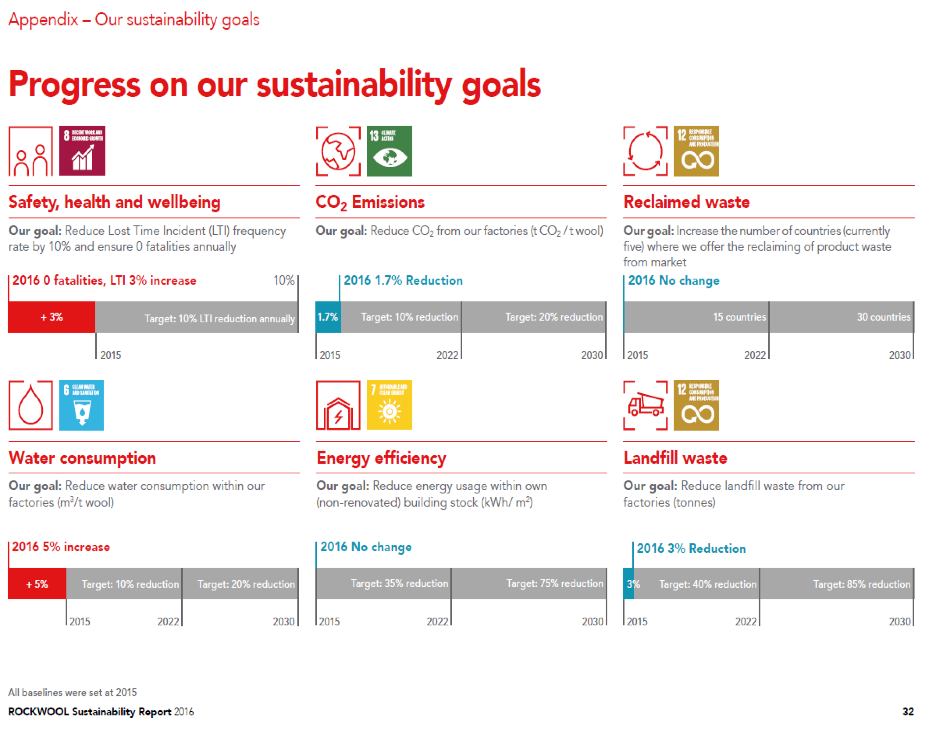
\includegraphics [scale=0.9]{bilder/baerkraftsmal.png}
\caption{Bærekraftsmål}
\label{fig:baerkraftsmal}
\end{figure}

\section{Markedet i Norge}  
Byggisolasjonsbransjen består av noen få store aktører som i likhet med Rockwool er datterselskaper av verdensomspennende konsern. Markedet karakteriseres av store mobilitetsbarrierer gjennom krav til kapitalintensive investeringer i spesialisert produksjonsutstyr. Rockwool har i flere år levert gode resultater, og er i dag markedets nest største aktør med en markedsandel på rundt 26\%. De mest nærliggende konkurrentene er Glava, Knauf, Sundolitt og Paroc, hvor Glava er markedets største med en markedsandel på 40\%. Kundene består i hovedsak av byggevarekjeder og entreprenører og sitter med høy forhandlingsmakt i form av at produsentene tilbyr lite differensierte produkter. Imidlertid leverer Rockwool og Paroc de mest differensierte produktene i form av produktegenskapene. De to virksomhetene er de eneste produsentene som leverer produkter som isolerer, er vannavstøtende, har lyddempende egenskaper og som er en god kilde til brannsikring. 

\indent \newline
Markedsveksten ligger på rundt 2\% og forventes å ligge på samme nivå i årene fremover. Dette viser til et modent marked. Den siste tiden har imidlertid Rockwool opplevd en lavere prosentvis vekst, grunnet en utvikling i markedet hvor miljøet blir vektlagt mer enn tidligere. Det blir vanligere for entreprenørene å BREEAM-sertifisere prosjektene sine. BREEAM er et miljøsertifiseringsverktøy for bygninger som legger vekt på miljøpåvirkning innenfor emner som energibruk, transport, materialer, avfall og forurensning\cite{breeam}. Dette påvirker spesielt produksjonsprosessen til isolasjonsprodusentene ved å stille krav til lavere utslipp. Rockwool sin nåværende smelteteknologi gir et høyere utslipp enn flere av konkurrentene, og er dermed en svakhet for virksomheten i forhold til å bli en foretrukken leverandør. 

\indent \newline
Det finnes også et annet økonomisk insentiv for produsentene til å redusere CO2-utslippet. Gjennom EØS-avtalen er Norge en del av Det europeiske kvotesystemet. Produsentene blir tildelt et visst antall kvoter og må kjøpe mer hvis utslippet overskrider det de får tildelt. Reduksjon i CO2-utslipp vil derfor resultere i lavere kostnader knyttet til drift.

\chapter{Beslutningsalternativer}
\section{El-ovn}
Rockwool besluttet i desember 2018 å investere i en ny smelteovn som vil benytte elektrisitet som energikilde. Beslutningen ble tatt etter å ha fått godkjent søknaden om 101,5 millioner kroner i støtte fra Enova. Enova er forvalter av Energifondet, og støtter norske bedrifter som ønsker en omstilling til lavutslippssamfunnet \cite{enova}. En elektrisk smelteovn er ikke tilgjengelig i markedet i dag, og investeringen krever at Rockwool selv utvikler nye og hensiktsmessige teknologiske løsninger tilpasset egen produksjon. Beregninger foretatt av selskapet viser til et investeringsbeløp på ca. 340 millioner kroner som fordeles i 2018, 2019 og 2020. Beløpet gjelder investeringer i innovasjon, teknologi og personalopplæring. 

\indent \newline
En el-ovn forventes å håndtere opp til 40\% gammel steinull (resirkulering), med en kapasitet på rundt 11.000 tonn steinullavfall fra byggeplasser. Dette tilsvarer mer enn totalt deponi av steinull per år fra byggmarkedet. Norge er i en særstilling når det gjelder avfall, hvor avfall til deponi, både fra produksjon og byggeplass, har vært relativt billig i flere år. Situasjonen er imidlertid i ferd med å endre seg da nye markeds- og myndighetskrav forventes fremover. Avfallet fra produksjonen representerer stangmøllemel (granulert ull) og små mengder avfall/kapp av ny isolasjon som returneres fra markedet. Øvrig produksjonsavfall består av ovnsbunn (jern, slagger og fines) og flyveaske. Teknologien vil kunne føre til en avfallsreduksjon på 19.677 tonn per år. Det tilsvarer en reduksjon på ca. 95\% sammenlignet med 2017.

\begin{table}[H]
  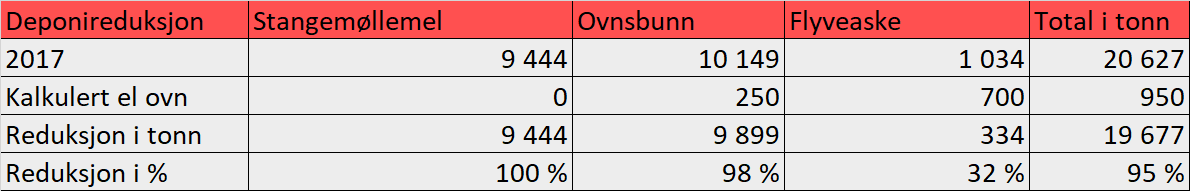
\includegraphics[width=\linewidth]{tabeller/deponireduksjon.png}
  \caption{Deponireduksjon}
  \label{tbl:deponireduksjon}
\end{table}

\indent \newline
Konvertering fra koks til elektrisitet vil også føre til store endringer med tanke på CO2-utslippet. Analyser fra Rockwool viser til en potensiell reduksjon i CO2-nivå med omtrent 80\%. Investeringen vil dermed føre til reduserte kostnader i forbindelse med CO2-kvoter, deponi og resirkulering. 

\begin{table}[H]
  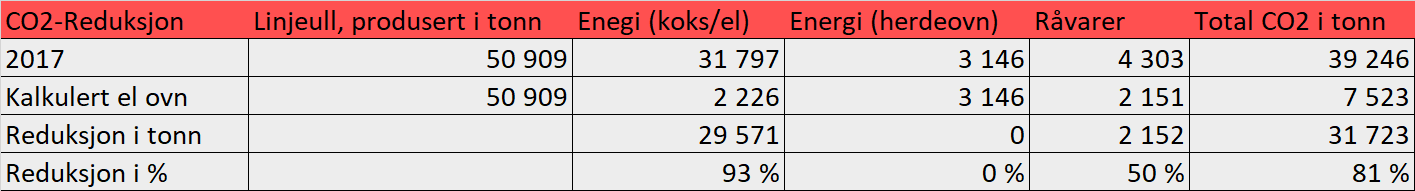
\includegraphics[width=\linewidth]{tabeller/co2reduksjon.png}
  \caption{CO2-reduksjon}
  \label{tbl:co2reduksjon}
\end{table}

\indent \newline
Investeringen baserer seg på utvikling innenfor teknologi og innovasjon i fire hovedelementer;

\begin{itemize}
\item[1.] Sikkerhet - Bygge den hittil største Submerged Arc Furnace (SAF) med lite smelteblad. En normal SAF-ovn med ønsket charge rate på 11,5 tonn per time vil ha en diameter på 8-9 meter og holde 189 tonn smelte. For å redusere risiko skal denne reduseres ned til 5,5-6 meter og holde 73 tonn smelte. Dette innebærer at en ny ovnstype med høyere “loadfaktor” må utvikles, noe som gir en høyere termisk belastning på ovnen og oppmuringsmaterialer.

\item[2.] Utvikle en SAF som kan håndtere en høy last samtidig med høy resirkuleringsandel. Dagens el-ovner har en begrensning i load og resirkuleringsfaktor, det vil si enten en høy load og lav resirkulering eller lav load og høy resirkulering. En resirkuleringsandel på 40\% vil stille nye krav til røykgassrensning. Resirkulert steinull inneholder mer organisk materiale sammenlignet med kun bruk av stein som råvare. Mengden rørgasser forventes derfor å øke sammenlignet med dagens produksjon.

\item[3.] Temperaturstabilitet - Utvikle en ny homogeniseringskanal.Fra ovn til spinnemaskiner er det over tre meter. Det ligger utfordringer i å sikre en stabil smeltetemperatur til spinnemaskinene. Det må derfor utvikles en homogeniseringskanal mellom ovn og eksisterende spinnere, da en slik kanal ikke er tilgjengelig i dag. Ved å sikre en stabil temperatur på +/- 10 grader celcius vil kanalen resultere i et høyere spinneutbytte.

\item[4.] Utvikle rett sammensetning av lining og effektivisere liningsbyttet. En høy grad av resirkulering vil stille nye krav til isolasjonsmateriale på innsiden av ovnen (lining). En ingeniørgruppe i Rockwool arbeider med å utvikle den rette sammensetningen for riktig lining. Erfaring viser at resirkulering øker slitasjen på liningen. Dette vil påvirke vedlikeholdsintervallene ved å gå fra hvert tredje år til hvert andre år. Målet er å redusere tiden det tar å skifte lining fra 3-4 uker til under 2 uker.
\end{itemize}

\indent \newline
I forbindelse med dimensjoneringen av smelteovnen vil selskapet produsere i et kapasitetsområde som ikke er prøvd ut tidligere. Overdimensjoneringen vil øke investeringen og risikoen i prosjektet, men anses som nødvendig for å opprettholde produksjonskapasiteten i Moss. Hvis temperaturstabillitet ikke oppnås, kan avfallsprosenten stige eksplosivt til 10-15\%. En marginal endring på 1\% resulterer i økte kostnader på 1,2 millioner kroner. Dette er isolert sett den største risikoen i prosjektet.

\indent \newline
I tillegg påløper det risiko knyttet til drift i form av en situasjon hvor det ikke oppnås full effekt. Dette fører til at resten av produksjonsanlegget ikke anvendes optimalt i forhold til produksjonsvolumene det er tilpasset til. Det vil også med stor sannsynlighet oppstå hyppigere og lengre stopp i produksjon, spesielt med tanke på liningslitasje. 

\section{Nåværende smelteteknologi}
Smelteteknologien som blir brukt i dag er en kupolovn, hvor energibærerne hovedsakelig består av koks og kalsinert karbon. Råvarer som benyttes er Anortositt, Gabbro, Fundia slagg, Dolomitt og Merox slagg. Per i dag har ikke kupolovnen nødvendig teknologi til å håndtere avfall fra byggeplasser.

\indent \newline
Å basere produksjonen hovedsakelig på fossile energibærere kan være risikofullt og kostbart, da markedsutviklingen går mot grønnere produkter. Klimarisikoen kommer til syne på et overordnet nivå, i form av Paris-avtalen og FNs bærekraftsmål, og på et underordnet nivå, i form av krav fra byggherrer og entreprenører. Rockwool har allerede erfart dette ved at byggaktørene har begynt å velge produkter som har et lavere CO2-avtrykk. Dette er gitt at øvrige byggetekniske krav er ivaretatt og prisen er konkurransedyktig. 

\indent \newline
Fokus på sirkulær økonomi har også fått større betydning de senere årene. Byggavfall er en stor kilde til avfall, og det forventes at markedet på sikt vil stille strengere krav til materialgjenvinning. I følge Erik Ølstad har eksempelvis Statsbygg signalisert at Rockwool må forberede seg på å endre dagens praksis og være i stand til å ta i mot retur av steinullavfall i fremtiden. 

\section{Brun smelteteknologi (BAT)}
En alternativ investering er en IMF-ovn (fluid bed ovn) hvor energibæreren er kull eller gass. Dette er en BAT-løsning (Best Available Technology) som kan bli gjennomført basert på Rockwool-konsernets egen smelteteknologi. Investeringen ligger på ca. 5 millioner kroner og innebærer redusert ovnsbunn og installasjon av full innvendig lining. Kostnaden for en slik smeltelinje ligger på samme nivå som en elektrisk smeltelinje. Imidlertid vil en BAT-oppdatering maksimalt resultere i 20-30\% CO2-reduksjon. Dette er derfor ikke en bærekraftig investering med en 10-års horisont. Høye vedlikeholdskostnader vil i tillegg gjøre det vanskelig for Rockwool å finansiere en slik løsning, da kapasiteten i Moss ikke er stor nok. I følge Rockwool var dette ikke et reelt alternativ, og beslutningen stod mellom å investere i el-teknologi eller å fortsette med nåværende teknologi. Vi vil på bakgrunn av dette ikke gå videre med å undersøke lønnsomheten av dette alternativet.


\chapter{Metode}
Metode omhandler aspekter knyttet til hvordan man går frem for å skaffe seg kunnskap. [Genaro Sucarrat; metode og økonometri].
\indent \newline
Metode er viktig i utredningen av økonomiske problemstillinger/analyser ettersom det spiller en sentral rolle i forberedelsene, gjennomføringen og tolkningen av undersøkelsene. I tillegg til å sikre god gjennomføring av egne analyser skal metodelæren bidra til å kunne evaluere styrker og svakheter ved andres undersøkelser. Metodelæren skilles i kvantitativ og kvalitativ metode. Kvantitativ metode tar sikte på å forklare eller anslå, mens kvalitativ metode tar sikte på å forstå.
Vi har benyttet oss av primær- og sekundærdata som er innhentet gjennom kvantitative og kvalitative metoder. Primærdata blir omtalt som data som blir hentet til et spesifikt formål, mens sekundærdata er data som allerede eksisterer og gjerne har tjent et annet formål tidligere.
 
\section{Kvantitativ metode}
For å utrede en netto nåverdianalyse har vi vært avhengig av historiske regnskapstall så vel som rent tekniske tall knyttet til produksjon og anslag rundt den nye smelteovnen. Rockwool har sendt oss en rekke dokumenter der vi har hentet ut relevante tall. Vi har brukt tallene for å modellere kontantstrømmer, avkastningskrav og sensitivitetsanalyser i Excel. Foruten innsikten fra Rockwool har vi brukt Proff-Forvalt, Norges Bank, NVE, samt flere relevante nettsider for å redegjøre for makroforhold og andre relevante beregninger.
 
\section{Kvalitativ metode}
Erik Ølstad, fabrikksjef i Moss, har vært vår kilde for innhenting av primærdata. Vi har ved flere anledninger møttes for uformelle samtaler der vi har fått belyst relevante spørsmål. Innsikten fra Erik har vært svært hjelpsom, både i form av kvantitative analyser, men han har også gitt oss en solid forståelse for markedet Rockwool opererer i.   
 
\indent \newline
Ref Genaro Sucarrat; [metode og økonometri- en moderne innføring 2. utgave]. Fagbokforlaget 2017.


\chapter{Teori}
\section{Netto nåverdimetoden}
Vi har i denne oppgaven valgt å besvare problemstillingen i lys av netto nåverdimetoden, da investeringen krever en flerperiodisk analyse (Espen Skaldehaug. forelesningsnotater/veiledningstime). Netto nåverdimetoden finner lønnsomheten til en investering ved å neddiskontere nåverdien av de fremtidige kontantstrømmene. Til tross for at NNV er den anbefalte metoden byr den på utfordringer. Estimering av fremtidige kontanstrømmer er i utgangspunktet umulig, men med fornuftige forutsetnigner og god markedsforståelse er det mulig å gjøre presise anslag. 

\indent \newline
\begin{math}
NNV={-X_0} + \frac {Xn}{1+r^n}
\end{math}

\indent \newline
Metoden belyser viktige momenter rundt tidshorisont og usikkerhet. Kroneverdien vil endres over tid, dette kan forklares med at man alternativt kunne plassert pengene der de vil forrente seg, inflasjon, og det faktum at det i prosjekter er knyttet usikkerhet til de fremtidige kontantstrømmene, og man vil ha kompensasjon for dette. Avkastningskravet vil hensynta denne usikkerheten. 

\indent \newline
En normal antakelse i forbindelse med bruk av netto nåverdimetoden er at man ønsker å maksimere eiernes profitt. Med bakgrunn i dette sier teorien at man alltid skal akseptere prosjekter med netto nåverdi > 0. I praksis vil dette bety en ekstraordinær avkastning på investert kapital. Dersom svaret blir positivt krever dette forklaring, gjerne gjennom effisiens-begrepet. 

\subsection*{Totalkapitalmetoden}
For å finne kontantstrømmen som skal tilkomme både eiere og långivere brukes totalkapitalmetoden. Metoden tar i bruk kontantstrømmen fra driften, finansielle poster utelukkes (Bøhren, Michalsen, Norli. S.351). Avkastningskravet skal reflektere avkastningen man alternativt kunne oppnådd ved å plassere midlene et annet sted med lik risiko (eStudie). WACC (Weighted average cost of capital) blir det relevante avkastningskravet ettersom modellen hensyntar investeringens finansiering gjennom en vekting av egenkapitalen og gjelden.

\[kT = kE * \frac{E}{E + G} + kG * (1-S) * \frac{G}{E + G}\]

\textit{hvor:
\begin{itemize}
    \item[] $kT$ = totalkapitalkostnaden etter skatt
    \item[] $kE$ = egenkapitalkostnaden etter skatt
    \item[] $kG$ = effektiv lånerente før skatt
    \item[] $s$ = relevant skattesats
    \item[] $E$ = egenkapitalens markedsverdi
    \item[] $G$ = gjeldens markedsverdi
\end{itemize}
}

\subsection*{Egenkapitalmetoden}
I egenkapitalmetoden er målet å finne kontantstrømmen til eierne. Sammenlignet med totalkapitalmetoden vil vi nå justere telleren for gjeldsopptak, renter og avdrag, inklusive renteskattefordelen (Bøgren, Michalsen, Norli. S.351). Kontantstrømmen vil så neddiskonteres med et avkastningskrav som reflekterer eiernes finansielle risiko. Det relevante avkastningskravet ved bruk av denne metoden er CAPM (Capital Asset Pricing Model).

\[kE = rf * (1-S) + \beta ek * [E(rm)-rf * (1-S)] \]

\textit{hvor:
\begin{itemize}
    \item[] $kE$ = egenkapitalkostnaden etter skatt
    \item[] $rf$ = risikofri rente
    \item[] $\beta ek$ = egenkapitalbeta
    \item[] $E(rm)$ = forventet avkastning på markedsporteføljen
    \item[] $s$ = skattesats
\end{itemize}
}
https://www.reuters.com/finance/stocks/overview/ROCKb.CO

\subsection{Estimering av risikofri rente \texorpdfstring{$(rf)$}{}}
Risikofri rente er avkastning en investor kan forvente å få uten å påta seg risiko. Et mål som ofte blir brukt på risikofri rente er statsobligasjoner. Den eneste måten man ikke skal kunne få denne avkastningen er hvis staten ikke klarer å betale sine forpliktelser. Rentenivået varier med løpetiden til statsobligasjonene, og det er derfor hensiktsmessig å velge rente på statsobligasjoner som er relevant for prosjektets levetid. Vi benytter derfor en effektiv rente på 10-års statsobligasjoner som risikofri rente. Per april 2019 var denne 1,71\%. https://www.norges-bank.no/tema/Statistikk/Rentestatistikk/Statsobligasjoner-Rente-Manedsgjennomsnitt-av-daglige-noteringer/

\subsection{Markedets risikopremie \texorpdfstring{$[E(rm) - rf *(1 - s)]$}{}}
Markedets risikopremie er den meravkastningen man krever ved å påta seg risiko. For å gjøre beregninger rundt dette er det nødvendig å se på de historiske dataene, da det ikke finnes noen god modell for å beregne fremtidige risikopremier. Fra 1976-2015 var den årlige norske risikopremien på 6,4\% (finansboka), men trenden de siste 20 årene har dog vært avtakende. PwC ferdigstilte i desember 2018 sitt mål for markedspremien, og denne lå på 5\%. Dette blir også vårt grunnlag for beregningen videre. 

https://www.pwc.no/no/publikasjoner/risikopremien-2018.html

\subsection{Estimering av betaverdi \texorpdfstring{($\beta ek$)}{}}
\[kE = rf * (1-S) + \beta ek * [E(rm)-rf * (1-S)] \]
\[0,0171 * 0,78 + 0,7 * (0,05 - 0,0171 * 0,78)= 3,9\%\]

\subsection{Blumes justeringsmodell}
Analyser gjennomført av Marshall Blume viser at selskapers BETA-verdier tenderer å bevege seg mot 1, og at selskaper med BETA-verdier nærme 1, er mer stabile enn de som er lengre unna. Blume mente derfor at det er hensiktsmessig å justere betaen ved følgende modell:

\[\beta justert = \beta raw * P +1,0 *(1-P)\]
Nyere forskning viser til at dette er fornuftig, derfor vil vi justere betaen for “mean reversion”. (forelesningsnotater “beregning av avkastningskrav” Pål Bertling-Hansen)

https://www.magma.no/hvordan-handtere-landrisiko-ved-investeringsbeslutninger1
https://www.infrontanalytics.com/fe-en/30064SD/Rockwool-International-A-S/Beta

\subsection{Beregning av egenkapitalens avkastningskrav (CAPM)}
\subsection{Totalkapitalens avkastningskrav}
\subsection{Internrentemetoden}
Internrentemetoden viser hvilket avkastningskrav som vil gi en avkastning på null i en netto nåverdiberegning. Metoden vil i vår oppgave kun bli brukt til å belyse hva som vil være høyeste mulig avkastningskrav for en lønnsom investering, da alle avkastningskrav høyere enn denne vil gi en negativ nåverdi.  

\subsection{Konsistensbetingelser}
En forutsetning for at netto nåverdimetoden skal forme et realistisk bilde av lønnsomheten i prosjektet er at konsistensbetingelsene legges til grunn. Med dette menes blant annet at man har frihet til å velge nominelle eller reelle tallstørrelser før eller etter skatt så lenge valgt metode er lik i teller og nevner. Vårt standpunkt tar utgangspunkt i de 5 grunnleggende konsistensbetingelsene (Forelesningsnotater).

\begin{itemize}
\item Nominelle tall - Tallene vi bruker vil være nominelle, altså vil inflasjon være hensyntatt. 
\item Etter skatt: Utregning av kontantstrøm og avkastningskrav vil bli beregnet etter fratrukket skatt ettersom skattereduksjonen aldri er lik i teller og nevner (forelesningsnotater).
\item Periodelengde: Teknisk levetid på investeringen vil antas å ha en levetid på 10 år, mens den økonomiske levetiden er antatt å være 20 år.
\item Kontantstrømmen: Bruke TK og eller EK ?
\item Risiko: Ettersom investeringen er av en ny teknologi som tidligere ikke er utprøvd foreligger det usikkerhet vedrørende investeringen. Usikkerheten knyttet til kontantstrømmene vil bli synliggjort i avkastningskravet. 
\end{itemize}

\subsection{Markedseffisiens}
Netto nåverdinalysen blir ikke tilstrekkelig uten å redegjøre for effisiensbegrepet. Et effisient marked betyr at all informasjon er priset inn i markedet. Dersom dette er sant vil det ikke være mulig å oppnå en ekstraordinær avkastning utover avkastningskravet. 
En NNV>0 betyr at investeringen har gitt en ekstraordinær avkastning.  

\subsection{Stikkord}
Effisient marked: Prisene reflekterer all relevant informasjon, NNV>0 er utenkelig, kontantstrømmen regnet for høy eller avkastningskravet for lavt, kombinasjon.
Ineffisient marked: AS ROCKWOOL vet noe de andre ikke vet (informasjonen varer ikke evig). Kan ha hef10 konkurransefortrinn. 






\chapter{Makroøkonomiske forhold}
\section{Inflasjon}
Inflasjon er nødvendig å ta hensyn til ettersom pengeverdien i en flerperiodisk analyse vil forandre seg over tid. Å gi et korrekt anslag av hvordan dette vil utvikle seg i årene fremover er vanskelig på grunn av usikkerhet i markedet, men vi legger til grunn prognoser fra Norges Bank som anslår en fremtidig inflasjons økning på 2\%. Tolvmånedersendringen (Mars 2018- Mars 2019) ligger på 2,9\%, men er ventet å synke de kommende årene \cite{inflasjon}.

\section{Utvikling i norsk økonomi}
Norsk økonomi er inne i en oppgangskonjunktur. I 2018 var BNP-veksten 1,4\%, og det forventes at veksten i 2019 vil øke til 2,3\% basert på forrige år. Bakgrunnen for de gode tallene er økt sysselsetting, høy aktivitet i flere bransjer og investeringene i fastlandsbedriftene har ikke vært høyere på 10 år. I motsetning til Norge har veksten i flere land i Europa avtatt den siste tiden, noe som kan føre til lavere etterspørsel etter norske varer. 

\indent \newline
Økte boligpriser har gjort boligbygging mer lønnsomt de siste årene. Dersom oppgangskonjunkturen i Norge fortsetter, noe som bidrar til økte inntekter, kan dette tale for enda flere boligutbyggelser. Derimot taler renteheving og lavere befolkningsvekst mot dette. Dette gir grunn til å anslå den fremtidige veksten i bygg- og anleggsbransjen til å være relativt moderat \cite{norskokonomi}.

\section{Økende fokus på miljø}
De siste årene har fokus på miljø blitt viktigere, både på et globalt- og nasjonalt nivå. I 2015 vedtok medlemslandene i FN 17 mål for bærekraftig utvikling som varer frem til 2030. Flere av målene omhandler å bekjempe klimaendringene og konsekvensene av dem. Dette gjelder spesielt reduksjon i utslipp av klimagasser. Der mange virksomheter tidligere ikke har måtte ta hensyn til utslipp og bærekraftig produksjon, har dette blitt en viktig del av hverdagen, og spesielt fremtiden. I tillegg til å jobbe mot FNs bærekraftsmål har Norge forpliktet seg til å oppfylle Parisavtalen. På bakgrunn av dette stilles det strengere krav til norske virksomheters CO2-fotavtrykk i form av både utslipp og avfall (deponi). Det forventes at kravene vil øke med tiden \cite{baerekraftsmaal}.

\subsection{Klimakvoter}
Klimakvoter er tillatelser til å slippe ut en viss mengde klimagasser. Disse blir som regel målt i tonn. Norge har gjennom EØS-avtalen vært en del av Det europeiske kvotesystemet siden 2008. I et kvotesystem finnes det et bestemt antall kvoter som kan selges og kjøpes. Antall tilgjengelige kvoter reduseres over tid med et formål om å kutte totalutslippet av klimagasser. Det europeiske kvotesystemet omfatter om lag 140 norske virksomheter innenfor industrier som gass- og kullkraftverk, energianlegg, petroleumsutvinning og offshoreanlegg, raffinerier, treforedling, jern- og stålproduksjon, ferrolegeringer, aluminium, mineralgjødsel, sement og kalk. Norge og EU har gjennom Paris-avtalen forpliktet seg til å redusere klimautslippene med minst 40 prosent regnet fra 1990 til 2030, og redusere utslippene i det europeiske kvotesystemet med 43 prosent fra 2005 til 2030.

\indent \newline
Reduksjonen foregår ved å senke taket på det totale antall kvoter i systemet. Knapphet på kvoter skaper dermed en markedspris på utslippene, hvor en høyere pris skaper insentiv til å redusere utslippene. I praksis kan en virksomhet som klarer å redusere utslipp til et nivå som gir dem et overskudd av kvoter selge disse til andre virksomheter som ligger på et høyere nivå enn tildelte kvoter. Fra 2010 har nedskaleringsfaktoren ligget på 1,74 prosent og vil gjelde ut 2020. Fra og med 2021 vil faktoren øke til 2,2 prosent per år og dermed skape større press på de kvotepliktige virksomhetene til å kutte utslipp \cite{klimakvoter}.

\indent \newline
Antall tilgjengelige kvoter i systemet påvirker prisen per kvote. Fra 2010 frem til 2018 har prisen omtrent ligget mellom 5 og 15 euro. Imidlertid har prisen økt kraftig de to siste årene og ligger per mai 2019 på 25 euro. Den kraftige økningen er ventet å fortsette, spesielt i årene etter 2021 hvor den nye nedskaleringsfaktoren tas i bruk \cite{kvotemarked}.
Figuren under viser rockwool sitt co2-utslipp (rød graf) og tildelte kvoter (grønn graf) i perioden 2012-2017.

\begin{figure}[H]
  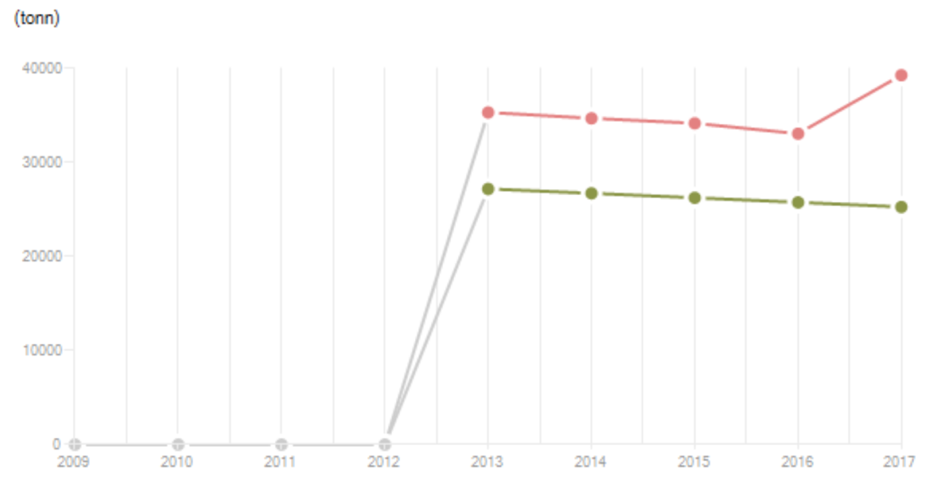
\includegraphics[width=\linewidth]{bilder/co2utslipp.png}
  \caption{Rockwool kvote og co2-utslipp - \cite{utslippkvote}}
  \label{fig:co2utslipp}
\end{figure}

\subsection{Avfall/resirkulering}
I 2015 presenterte Europakommisjonen et forslag til en ny sirkulær-økonomi pakke som blant annet omhandler endring av avfalls - og resirkuleringsregelverket. Målet med forslaget er å bedre den miljømessige samfunnsutviklingen gjennom effektivisering av ressursbruk gjennom hele verdikjeden (produksjon, forbruk og avfallsbehandling). En sirkulær økonomi er basert på gjenbruk, reparasjon, oppussing/forbedring og materialgjenvinning hvor færrest mulig ressurser går tapt \cite{sirkularokonomi}.

\indent \newline
Videre ble det i 2018 vedtatt endringer i deponidirektivet som er en del av sirkulær-økonomi pakken. Endringene omhandler strengere krav og begrensninger på avfall som tillates deponert. Dette gjelder spesielt avfall som egner seg for materialgjenvinning \cite{materialgjenvinning}.

\section{Kraftpriser}
Den nye smelteovnen til Rockwool vil bruke elektrisitet som energikilde, noe som krever økt strømforbruk. I den forbindelse er det viktig å gjøre anslag om hvordan strømprisen kan endres gjennom investeringens levetid.

\indent \newline
Det er flere faktorer som ligger til grunn for strømprisen i Norge. De viktigste er værforholdet, etterspørsel, kull- og gasspriser og prisen på CO2-kvoter. Norge er koblet opp mot det Europeiske kraftmarkedet, noe som fører til at svingninger i pris og produksjon i utlandet vil påvirke prisene i Norge. Krafthandlene gjøres gjennom Nord Pool AS, et aksjeselskap som eies av de nordiske og baltiske stamnettoperatørene.

\indent \newline
Været er den største forklaringskraften på hvor mye strøm Norge produserer hvert år. Basert på at omtrent 95\% av produsert elektrisitet kommer fra vannkraft vil nedbørsmengden ha stor innvirkning på eksport- og importbehovene til Norge. Anslag om fremtidige værutsikter er tilnærmet umulig, men man kan forutse en endring i klima basert på global oppvarming. Effekten av dette vil være vanskelig å forutse.

\indent \newline
Det er spådd en økning i etterspørselen etter elektrisitet i industri- og kraftmarkedet i fremtiden. Prognoser fra NVE (Norges Vassdrags- og Energidirektorat) viser til at norsk
industri kommer til å øke strømforbruket med omtrent 28\% fra 2018 til 2040. Dette
begrunnes med en økning i antall datasentre, og at flere industrier vil rette et større fokus mot en miljørettet profil.

\indent \newline
Ettersom Norge er koblet mot det Europeiske kraftmarkedet vil priser på kull og gass ha innvirkning på strømprisen i Norge. Store deler av produksjonen i Europa er preget av kullkraft, noe som betyr at en økning i kullprisen kan minske produksjonen i kullkraftverkene. Dette vil resultere i lavere kraftproduksjon, altså lavere tilbud, og økte priser. Det samme resonnementet gjelder CO2-kvoter.

\indent \newline
Historiske tall viser at strømprisen er relativt volatil. NVE estimerer fremtidig spotpris til mellom 36-37 øre pr kWh (Kilowattime) frem til 2030. Normalt vil det tillegges el-avgift og MVA på denne prisen. Relevant sats for disse er henholdsvis 0,48 øre per kWh for el-avgiften og MVA-satsen er på 25\%. El-avgiften for husholdninger er dog høyere, men industrinæringer har redusert sats.

\begin{table}[H]
  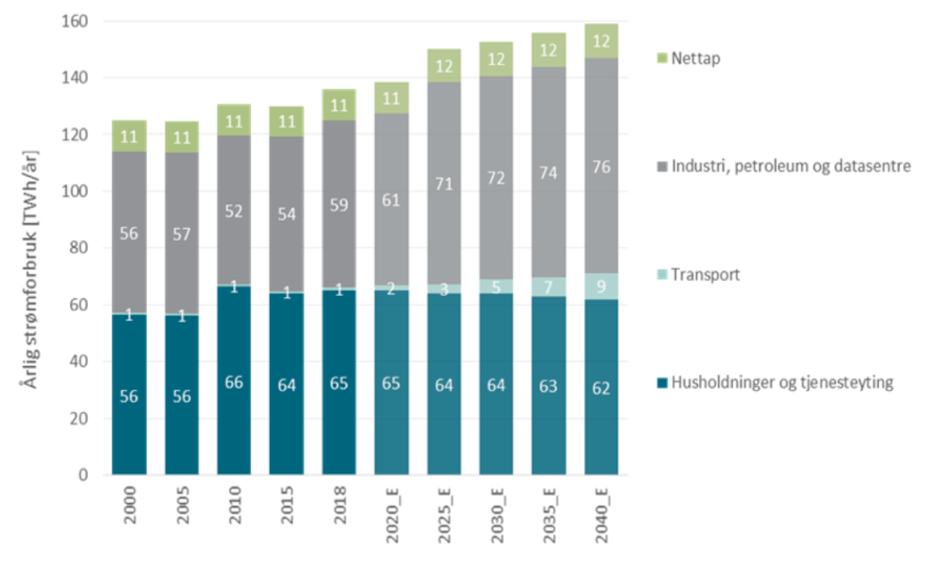
\includegraphics[width=\linewidth]{tabeller/stromforbruk.png}
  \caption{Strømforbruk - utvikling}
  \label{tbl:stromforbruk}
\end{table}

\begin{figure}[H]
  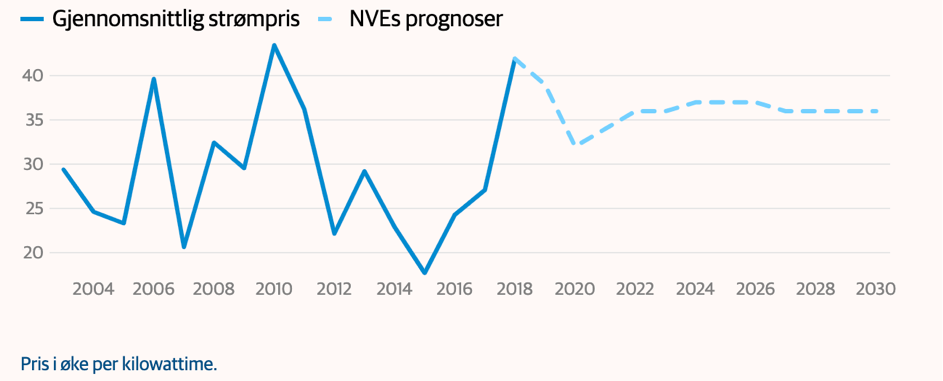
\includegraphics[width=\linewidth]{bilder/strompris.png}
  \caption{Strømpris - utvikling}
  \label{fig:strompris}
\end{figure}



 

\chapter{Spesifisering av data}
For å vurdere lønnsomheten av investeringen vil vi sammenligne kontantstrømmene prosjektet vil generere med nåværende teknologiløsning. Kapittelet vil presentere faktorer som legges til grunn for netto nåverdiberegningene.

\section{Grunnlag for beregning av netto nåverdi med el-teknologi}
\subsection{ Investering og finansiering}
Investeringen i el-ovnen koster totalt 340 millioner kroner, hvor investeringsbeløpet fordeler seg over årene 2018, 2019 og 2020 med henholdsvis 10,203, 136,035 og 193,850 millioner kroner. Enova bidrar med 101,5 millioner kroner i finansiell støtte, som dekker ca 39,1\% av investeringsbeløpene i hvert av årene. Resterende beløp på 238,5 millioner kroner finansieres med interne midler fra Rockwool-konsernet. Selve ovnen har en pris på 130 millioner kroner, hvor resten er tilleggsinvesteringer knyttet til installasjon og tilpasning av ovnen. 

\indent \newline
I følge Rockwool har investeringen en teknisk levetid på 10 år og en økonomisk levetid på 20 år. Den økonomiske levetiden vil derfor legges til grunn i analysen. Investeringen vurderes til å ha en utrangeringsverdi på 20\%, det vil si 47,7 millioner kroner. I utgangspunktet ønsker ikke konsernet å selge teknologien til konkurrerende aktører, så en mulig alternativ anvendelse av ovnen vil være å flytte den til en annen fabrikk i konsernet. Vi velger allikevel å tillegge investeringen en utrangeringsverdi større enn null, da muligheten for salg foreligger. 

\indent \newline
Det avsettes tre måneder sommeren 2020 til installasjon og omstilling til ny produksjonsteknologi. For å analysere investeringen over 20 hele perioder gjør vi en forenkling og forutsetter at produksjon med el-teknologi er i gang fra og med 2021.

\subsection{Driftsinntekter}
Inntektsberegningene tar utgangspunkt i salgsinntektene fra 2018. Det forventes en årlig markedsvekst på 2\%. Det ligger dermed et potensiale i markedet for å øke markedsandelen. Vi legger til grunn en nedgang i salgsvolum på 0,5\% i 2019 og 2020. Årsaken til dette er at markedet etterspør grønnere produkter. Fra og med 2021 vil vi bruke en vekst i salgsvolum på 1,5\% de 10 første årene basert på at Rockwool vil levere produkter med  det laveste CO2-avtrykket i markedet. Etter dette forventes det at flere aktører vil ha gått over til mer miljøvennlig produksjonsteknologi og veksten settes derfor til 0,5\%.

\subsection{Driftskostnader}
Varekostnader består av råvarer, energi, bindemiddel, renhold, deponi, CO2-kvoter, transport og direkte produksjonslønn. For å synliggjøre forskjellene mellom den nye og nåværende smelteteknologien har vi valgt å trekke ut kostnadene knyttet til strøm, koks, CO2-kvoter og deponi. Pris per utslippskvote ligger per mai 2019 på 245 kroner, og i følge Rockwool vil denne kunne øke til 400 kroner innen 2030. Dette resulterer i en årlig vekst på 5,75\%. I 2018 hadde virksomheten et CO2-utslipp på 39.246 tonn med tilhørende antall tildelte kvoter på 25.249. Med en reduksjon i CO2-utslipp på rundt 80\% vil Rockwool ha et overskudd av tildelte klimakvoter. I utgangspunktet kunne de ha solgt disse til andre kvotepliktige virksomheter, men fra og med 2021 innføres en ny ordning hvor tildelte kvoter baseres på foregående års utslipp. Ekstra inntekter vil derfor ikke forekomme, kun bortfall av kostnader. Strømprisen tillegges en vekst på 0,5\% og i forhold til deponi legges det til grunn en reduksjon på 95\%. Det forutsettes at produksjonsvolumet endrer seg i takt med salgsveksten. Driftskostnadene følger produksjonsvolumet.

\indent \newline
Lønnskostnader tillegges en årlig vekst på 2\% basert på reallønnsprognoser fra SSB \cite{reallonnsprognoser}.
Andre driftskostnader består av vedlikehold og faste kostnader. Investeringen krever hyppigere vedlikehold og gir en økt kostnad på 509.090 kroner.

\section{Grunnlag for beregning av netto nåverdi med nåværende teknologi}
\subsection{Driftsinntekter}
Grunnet økt etterspørsel etter grønnere produkter legger vi til grunn en nedgang i salgsvolum på 0,5\% i 2019 og 2020. Deretter deles de neste 20 årene inn i 5-års intervaller, hvor salgsvolumet reduseres med henholdvis 2, 3, 5 og 10\% per år i hvert intervall. Beregningene er basert på samtaler med Rockwool og utviklingen i markedet. 

\subsection{Driftskostnader}
Ved å fortsette med nåværende produksjonsteknologi vil virksomheten ha økte kostnader knyttet til koks, CO2-kvoter og deponi. Priser og tilhørende vekst behandles under samme forutsetninger som i punkt 8.1.3. Koksprisen forventes å følge inflasjon.

\section{Avskrivninger}
De regnskapsmessige avskrivningene behandles som lineære avskrivninger over en levetid på 20 år. Utrangeringsverdien er satt til 20\% av investeringskostnaden. Skattemessig skal varige driftsmidler avskrives etter saldometoden jf. skatteloven §§14-40 og 14-41. Avskrivningssatsen er på 20\% jf. skatteloven §14-43 første ledd bokstav d. Videre følger det av skatteloven §14-42 andre ledd bokstav a at bidrag fra offentlig støtte skal trekkes fra kostprisen ved utregningen. Dette medfører dermed at utgangspunktet for saldoberegningen blir kostpris fratrukket tilleggsstøtte fra Enova. Saldoavskrivningene legges til grunn ved beregning av skatt \cite{skatteloven}. 

\indent \newline
Den nåværende smelteovnen er allerede ferdig avskrevet, og vi vil på bakgrunn av dette kun hensynta avskrivningene knyttet til el-ovnen, da andre avskrivninger vil være like ved begge alternativene.

\section{Skatt}
Selskapsskatten i Norge ble endret fra 23\% til 22\% for 2019. Det er usikkerhet knyttet til hvordan denne vil endres i fremtiden. Flere instanser, som for eksempel NHO, ønsker å redusere skatten ytterligere, og viser til at Norge har høyere selskapsskatt enn nabolandene våre. Til tross for at også selskapsskatten har hatt en nedadgående kurve de senere årene velger vi å legge til grunn 22\% gjennom hele investeringens levetid. 

\indent \newline
Skatten skal i utgangspunktet betales i to like terminer i løpet av første halvår etter inntektsåret. For kontantstrømmen totalt sett vil det ikke ha betydning om vi trekker skatten etterskuddsvis eller ikke. På bakgrunn av dette legger vi til grunn at skatten utbetales samme år som den oppstår \cite{skattaksje}.

\section{Inflasjon}
Vi har valgt å sette inflasjonen lik 2,0\% i henhold til Norges Bank sine prognoser for fremtidig inflasjonsøkning. Vi benytter oss av nominell metode og vil derfor inflasjonsjustere driftsinntekter og driftskostnader.

\section{Arbeidskapital}
Nødvendig arbeidskapital beregnes av neste års omsetning og settes til 5\%. Estimatet er utarbeidet på bakgrunn av gjennomsnittlig endring i arbeidskapital de siste 5 årene og samtaler med Rockwool.





 

\chapter{Lønnsomhetsberegning - netto nåverdi}
For å vurdere lønnsomheten til prosjektet har vi utarbeidet kontantstrømmer prosjektet vil generere og kontantstrømmer basert på å fortsette med nåværende teknologi. Deretter har vi beregnet differansekontantstrømmer ved å sammenligne inntekter og kostnader de to alternativene medfører. Netto nåverdi-analysen baseres på sistnevnte beregning. Figuren nedenfor viser et utdrag fra differansekontantstrømmen i årene før el-ovnen er klar til produksjon, de første tre årene med produksjon og de to siste. Fullstendig kontanstrøm finnes i vedlegg ?.

\begin{table}[H]
  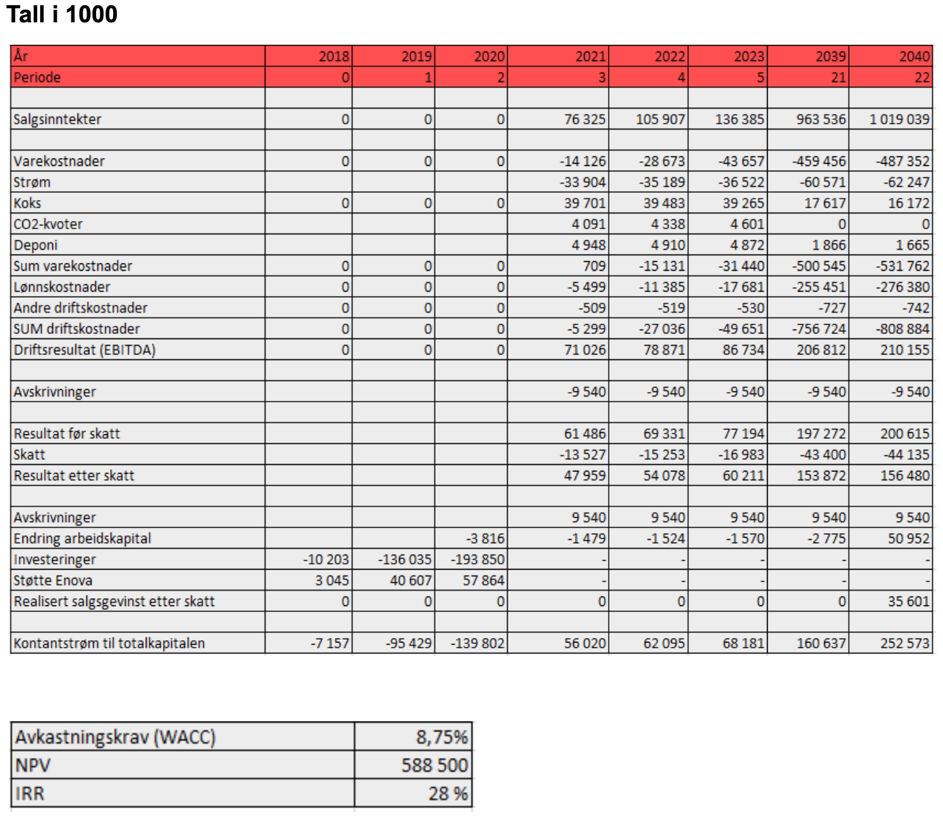
\includegraphics[width=\linewidth]{tabeller/lonnsomhet.png}
  \caption{Rockwool kontantstrømmer}
  \label{tbl:lonnsomhet}
\end{table}

Analysen viser til en positiv netto nåverdi på 588.500.000 kroner ved et totalkapitalkrav på 8,75\%. Den totale avkastningen på prosjektet er 28,32\% og vises gjennom internrenten. Dette gir en ekstraordinær avkastning på 19,57\% utover totalkapitalkravet.

\chapter{Sensitivitetsanalyse}
Ved å ta en rekke forutsetninger om fremtidig utvikling, inntekter, kostnader og makroforhold har vi kommet frem til et resultat vi mener gjenspeiler nåverdien av investeringen. Likevel foreligger det stor usikkerhet rundt momentene fremvist i oppgaven. Det vil derfor presenteres ulike fremtidsbilder av investeringen med formål om å avdekke nåverdien gitt nye forutsetninger. Dette vil først belyses gjennom en \textit{best case} og \textit{worst case} analyse, før vi deretter undersøker hvor stor påvirkning de mest usikre momentene vil ha på nåverdien.

\section{Best case}
I denne delen velger vi utelukkende å endre veksten i salgsvolumet. Grunnen til at vi velger å bruke salgsvolum som endringsvariabel er at den påvirker både inntektene og kostnadene, og beskriver den fremtidige utviklingen best. I best case analysen anslår vi at salgsvolumet øker med 3\% de første 10 årene, deretter vil salgsvolumet avta og ligge stabilt på 1\% gjenværende tid. Dette gir en økning i nåverdien på 340,491 millioner. Internrenten med denne forutsetningen økes fra 28\% til 36\%.

\section{Worst case}
Worst case analysen legger også til grunn vekst i salgsvolum som endringsvariabel. For å beskrive en fremtidig utvikling som vi anser som verst, men fortsatt realistisk, bruker vi en årlig negativ vekst i salgsvolumet på 2\% de første 10 årene, før den synker til 3\% per år resterende tid. Basert på disse estimatene vil investeringen gi en negativ netto nåverdi på 18,758 millioner kroner.

\begin{table}[H]
  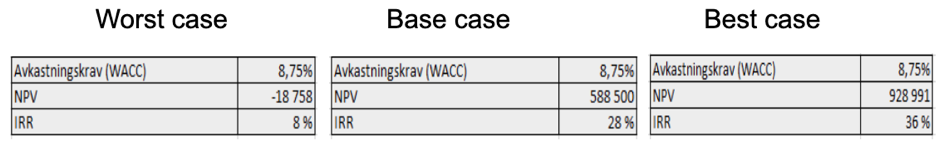
\includegraphics[width=\linewidth]{tabeller/case.png}
  \caption{Worst, Base og Best case oversikt}
  \label{tbl:case}
\end{table}

\section{Strømpris}
Strømprisen blir betraktet som en av de største merkostnadene til investeringen. Basert på historiske priser har denne vist seg å være ekstremt volatil, der man blant annet har opplevd en dobling i strømpris på kun ett år. Vår beregning tar utgangspunkt i en pris tilnærmet dagens nivå, med en økning på 0,25\% per år. Ved å endre denne prosentsatsen til 3\% vil netto nåverdien falle med omtrent 90 millioner. Investeringen vil fortsatt bli betraktet som svært lønnsom, og det er først ved en strømprisøkning på 10\% årlig at prosjektet gir en negativ avkastning.

\section{Totalkapitalkrav og levetid}
Avkastningskravet uttrykker usikkerheten i kontantstrømmene, og er derfor en av de mest utslagsgivende faktorene i vår analyse. Estimeringen av avkastningskravet har vært krevende å utforme, spesielt siden vi tillegger investeringen risiko utover selskapsrisikoen. Etter å ha utformet avkastningskravet basert på relevant teori kom vi frem til at investeringen hadde tilhørende risiko utover selskapets WACC. Vi behandlet dette ved å tillegge en prosentvis sats for henholdsvis business risk og valutarisiko. Ettersom disse satsene ble basert på skjønn er det nødvendig å foreta observasjoner av netto nåverdien der avkastningskravet settes både lavere og høyere enn det avkastningskravet vi har benyttet oss av.  

\begin{table}[H]
  \centering
  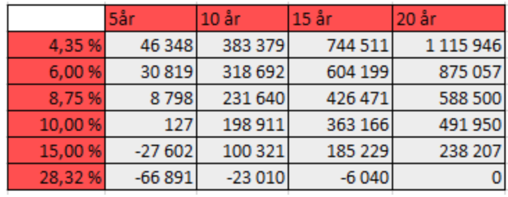
\includegraphics[scale=1.0]{tabeller/waccLevetid.png}
  \caption{WACC og levetid}
  \label{tbl:waccLevetid}
\end{table}

I tillegg til å legge inn nye avkastningskrav har vi også hensyntatt tidsperspektivet i denne analysen. I et fem-års perspektiv må avkastningskravet være 10\% for at investeringen ikke skal være lønnsom. Gjennom et 20-års perspektiv er investeringen lønnsom frem til og med internrenten som ligger på 28\%. Til tross for at lønnsomheten vil være positiv selv ved store endringer i avkastningskravet vil en endring på bare 1,25\% minske lønnsomheten med omtrent 100 millioner kroner. 

\section{Valutakurs}
Ettersom ROCKWOOL International er et multinasjonalt selskap, med hovedkontor i Danmark, vil kontantstrømmen kunne påvirkes av vekslingskursen mellom den norske og danske kronen. I modellen vår vil vi justere den estimerte nåverdien med diverse vekslingskurser. I tillegg til å bruke dagens kurs (Mai. 2019) har vi lagt ved ett utfall der den norske kronen svekkes mot den danske, ett der den norske kronen styrker seg mot den danske, og til slutt også gjennomsnittlig vekslingskurs de siste 5 årene, basert på månedlige observasjoner. I modellen legges det først til grunn at den danske kronekursen styrkes 10\% mot den norske, noe som fører til en ny netto nåverdi på 497,6 millioner danske kroner. Ved en dansk svekkelse med 10\% mot den norske kronen blir ny netto nåverdi 407,1 millioner danske kroner, noe som innebærer en differanse på omtrent 90 millioner danske kroner mot kronestyrkelsen. Dersom man legger til grunn en forventning om at den danske kronen vil ligne gjennomsnittet de siste fem årene vil netto nåverdien øke med omtrent 22 millioner for eierne. 


\begin{table}[H]
  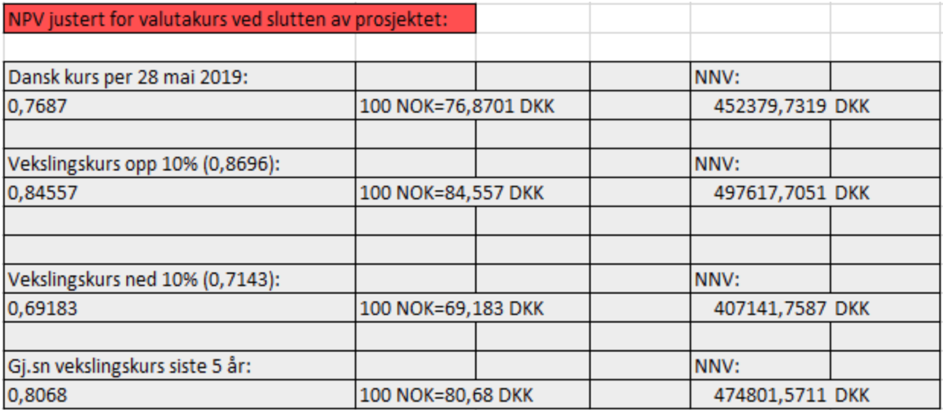
\includegraphics[width=\linewidth]{tabeller/NPVvaluta.png}
  \caption{NPV justert for valutakurs}
  \label{tbl:NPVvaluta}
\end{table}

\chapter{Drøfting}
I denne investeringsanalysen har vi beregnet netto nåverdi for to ulike alternativer for ROCKWOOL International, med et formål om å avgjøre om investeringen i ny el-smelteovn er lønnsom. Beregningene viser til en ekstraordinær avkastning på 19,57\% utover totalkapitalkravet, sammenlignet med alternativet som ville vært å fortsette med nåværende produksjonsteknologi. I et effisient marked er det i utgangspunktet ikke mulig å oppnå en slik ekstraordinær avkastning, og vi vil i det følgende diskutere årsaker som ligger bak dette, samt faktorer som er essensielle for lønnsomheten til prosjektet. 

\indent \newline
En viktig forutsetning for investeringens lønnsomhet er utviklingen i markedet. Det økende klima-fokuset, i form av FNs bærekraftsmål og Parisavtalen, skaper press på aktørene til å redusere utslipp i produksjonsprosessen. Dette forsterkes i tillegg av byggentreprenørenes økende bruk av BREEAM-sertifisering. Investeringen kan på grunnlag av dette karakteriseres som en strategisk beslutning med formål om å beholde dagens markedsandel og posisjon i Norge. Markedet er inne i en utvikling hvor produsenter som ikke tilpasser virksomheten til endringene vil kunne oppleve dramatiske fall i salgsveksten. Dette omtales ofte som “stall points”, og oppstår når aktører med gode markedsposisjoner ikke evner å oppfatte endring i markedsforutsetningene. Dette gjelder spesielt endring i kundenes verdivurdering av produktegenskapene. 

\indent \newline
Grunnen til at fabrikken i Moss ble valgt ut som pilotprosjekt er at det norske markedet oppfattes som det med størst press på de nevnte faktorene. I tillegg legger den norske politikken til rette for at virksomheter som ønsker å redusere utslippene kan få finansiell hjelp og støtte til å gjennomføre dette. I denne sammenheng var støtten fra Enova en viktig del av beslutningen. Sensitivitetsanalysen viser imidlertid at prosjektet gir en positiv netto nåverdi på 499,184 millioner kroner uten støtten på 101,5 millioner kroner, og er derfor ikke avgjørende for at prosjektet skal vurderes som lønnsomt. 

\indent \newline
Hovedårsaken til de store forskjellene i fremtidig kontantstrøm de to alternativene genererer er først og fremst veksten som legges til grunn. I alternativet med å fortsette med nåværende produksjonsteknologi vil virksomheten i Norge reduseres til en betydelig mindre aktør i markedet, mens den nye el-teknologien vil sørge for en fortsettelse av den stabile veksten virksomheten har opplevd i en årrekke. Det er også viktig å se på hvilke konkurransefortrinn investeringen gir. Sammenlignet med de andre konkurrentene vil Rockwool minimum redusere CO2-utslippet til samme nivå som Glava (markedsleder) ligger på i dag. De vil også oppnå et konkurransefortrinn i forhold til reduserte kostnader relatert til deponi. I dag prøver virksomheten å levere det mest differensierte produktet i form av produktegenskapene. Kostnadsbesparelsene vil kunne åpne opp for en ny virksomhetsstrategi i form av kostnadslederskap. Virksomheten vil derfor ha gode forutsetninger for å utfordre konkurrentene på pris.

\indent \newline
Imidlertid er det flere usikkerhetsmomenter knyttet til den nye teknologien, som kan påvirke lønnsomheten negativt. Innkjøringsperioden forventes å ta tre måneder, men siden teknologien ikke er testet ut i like stor skala tidligere, ligger det et usikkerhetsmoment ved at tilpasningen kan ta lenger tid enn forventet. Dette gjelder spesielt med tanke på å oppnå effektiv utnyttelse av ovnen og samsvar med øvrige deler av produksjonsanlegget. For å synliggjøre usikkerheten i prosjektet har vi gjennom sensitivitetsanalysen belyst hvordan endringer i de subjektive forutsetningene vil påvirke investeringens lønnsomhet. Det er vanskelig å forutse fremtidig utvikling i makrofaktorene, men analysen viser at det må forekomme ekstremutfall i forutsetningene for å gi en negativ netto nåverdi. Vi anser derfor investeringen som svært robust for uforutsette utfall.

\indent \newline
Avslutningsvis vil vi påpeke at investeringen kan skape verdier utover den positive netto nåverdien. Hvis pilotprosjektet viser seg å bli suksessfullt, vil investeringen gi selskapet verdifull kunnskap og erfaring til å imøtekomme de globale grønne markedsendringene. Investeringen kan potensielt være begynnelsen på endring av produksjonsteknologi blant alle fabrikkene til konsernet. Med en lenger tidshorisont enn vi har lagt til grunn i oppgaven forventes det et økende miljøpress i flere land. Vi anser derfor investeringen som en viktig beslutning med tanke på selskapets fremtidige utvikling, vekst og merkevare.


\chapter{Kritikk av oppgaven}
På grunn av oppgavens omfang har vi måttet foreta en rekke beregninger som i virkeligheten er umulig å spå. I tillegg har vi inkludert de momentene vi fant hensiktsmessig for å besvare problemstillingen best mulig. Det betyr likevel ikke at vi har fanget opp alle momentene som har relevans for å svare best mulig på oppgavens formål. 

\indent \newline
Avkastningskravet er en av beregningene som vil gi størst utslag på netto nåverdien. I analysen beregnet vi beta til ROCKWOOL International. Vi brukte dermed det danske konsernets korrelasjon til den danske børsen, men med tilhørende norsk risikofri rente og markedspremie. Dette kan ha ført til unøyaktige estimater, noe vi prøvde å ta høyde for ved å gjøre en ekstra beregning for sammenlignbare selskaper. I avkastningskravet har vi også lagt på ytterligere risiko etter WACC- beregningen var utført. Disse ble gjort med delvis skjønn og delvis gjennom samtaler med Rockwool. Anslaget kan være unøyaktig, og vil i så fall gi prosjektet feil risiko. 

\indent \newline
Regnskapstallene fra proff.no skilte ikke mellom produksjonsfabrikken i Moss og Trondheim. Dette førte til at vi ble nødt til å ta en forutsetning om hvor store deler av inntektene og kostnadene som hørte til hver fabrikk. Samtaler med Erik Ølstad indikerte at forutsetningen vår om å tillegge Moss ca 70\% av produksjonen var et realistisk anslag. Dette dannet dermed utgangspunktet for analysen vår, men disse kan avvike fra virkeligheten.

\indent \newline
Estimering av inntekter og kostnader har vært blant de mest krevende anslagene knyttet til oppgaven. Gjennom analysen har vi sammenlignet dagens drift med den nye investeringen for å estimere merinntekter og merkostnader som følge av prosjektet. Hvordan disse prisene faktisk vil utvikle seg i fremtiden er umulig å anslå. Vi har prøvd å forholde oss konsistente ved begge modellene, men det kan likevel ikke utelukkes at vi i beregningene har vært “bias” mot ett av alternativene. Videre har vi tatt høyde for at begge alternativene har en relevant tidshorisont på 20 år. I realiteten er det nærliggende å anta at bedriften ikke ville drevet ulønnsomt over flere perioder uten å endre strategi eller legge ned. 

\indent \newline
Flere av beregningen våre har tatt utgangspunkt i historiske tall til tross for at historien ikke nødvendigvis former et realistisk bilde av fremtiden. Sensitivitetsanalysen har som formål å synliggjøre hvordan beregninger avviker fra forutsetningene vi har lagt til grunn for vår analyse. 

\indent \newline
Vi har i aller høyeste grad forsøkt å stille oss kritiske til eget arbeid gjennom hele arbeidsprosessen for å forsikre oss om at vi har kommet frem til hensiktsmessige beslutninger. 


\chapter{Konklusjon}
Vi har utarbeidet en differansekontantstrøm over en periode på 20 år. Denne viser netto nåverdi av beslutningen om å investere i ny el-smelteovn, sammenlignet med å fortsette med nåværende smelteovn. Beregningene er basert på totalkapitalmetoden hvor relevant diskonteringsrente ble utarbeidet gjennom WACC med et risikopåslag knyttet til valuta og business risk. 

\indent \newline
Gjennom analysene våre har vi kommet frem til at investeringen vil være lønnsom, og generere en netto nåverdi på 588,500 millioner kroner. Den faktiske avkastningen på prosjektet er 28,32\% og gjenspeiler en avkastning på 19,57\% utover totalkapitalkravet. Sensitivitetsanalysen synliggjorde hvordan endringer i vekst og makroforhold vil påvirke prosjekts lønnsomhet. Resultatene viste til en svært solid investering, hvor det må forekomme ekstremutfall for at prosjektet ikke skal være lønnsomt. 

\indent \newline
Hovedårsaken til investeringens lønnsomhet ligger i markedsutviklingen, hvor prosjektet  legger til rette for at konsernets avdeling i Norge kan bevare dagens markedsposisjon og gi en stabil vekst i årene fremover. I alternativet med å fortsette med dagens løsning gir analysene grunn til å tro at Rockwool ville blitt en betydelig mindre aktør i det norske markedet.

\indent \newline
I tillegg til å generere en positiv netto nåverdi, vil pilotprosjektet i Moss styrke konsernets merkevare og støtte opp under selskapets utvalgte bærekraftsmål og visjon.

\indent \newline
Vi konkluderer med at beslutningen om å investere i en ny elektrisk smelteovn var lønnsom.


% chapter heading as preface and toc
\titleformat{\chapter}[display]
 {\bfseries\Large}
 {}
 {0pt}
 {\color{rockwoolcolor}\titlerule[2.0pt]\vspace{2ex}\filright\color{black}}
 [\color{rockwoolcolor}\vspace{2ex}{\titlerule[2.0pt]}]
 
\renewcommand\bibname{Referanseliste}
\bibliographystyle{apalike}	% (uses file "plain.bst")
\bibliography{mineReferanser}		% expects file "mineReferanser.bib"
}

\cleardoublepage
\renewcommand\appendixpagename{Appendiks}
\appendix
\appendixpage
\chapter{Rockwool beta regresjon}
\begin{figure}[H]
\centering

\includegraphics [scale=0.65]{appendiks/bilder/rockwoolbetaregfull.png}
\caption{Rockwool beta regresjon full}
\label{fig:rockwoolbetaregfull}
\end{figure}

\begin{figure}[H]
\centering
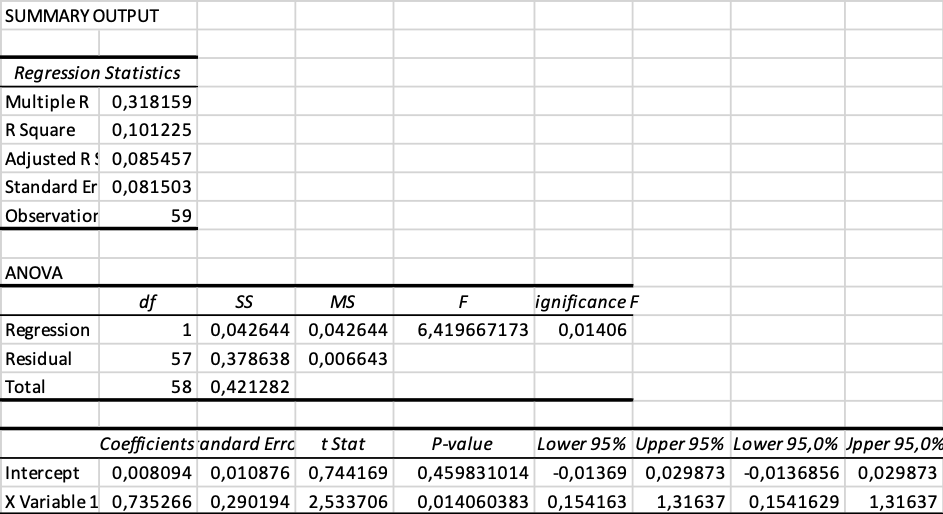
\includegraphics [scale=0.9]{appendiks/bilder/rockwoolbetaregsummary.png}
\caption{Rockwool beta regresjon oppsummering}
\label{fig:rockwoolbetaregsummary}
\end{figure}

\chapter{Rockwool avkastningskrav}
\begin{figure}[H]
\centering
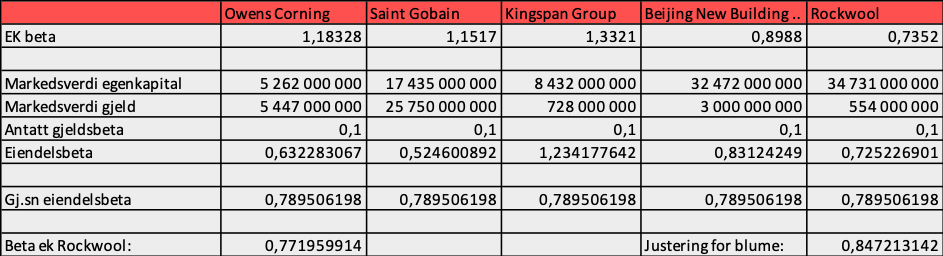
\includegraphics [scale=0.9]{appendiks/bilder/avkastningskrav.png}
\caption{Avkastningskrav - sammenlignbare selskaper \cite{yahoo}}
\label{fig:avkastningskrav}
\end{figure}

\chapter{Rockwool kontantstrømmer}
\begin{figure}[H]
\centering
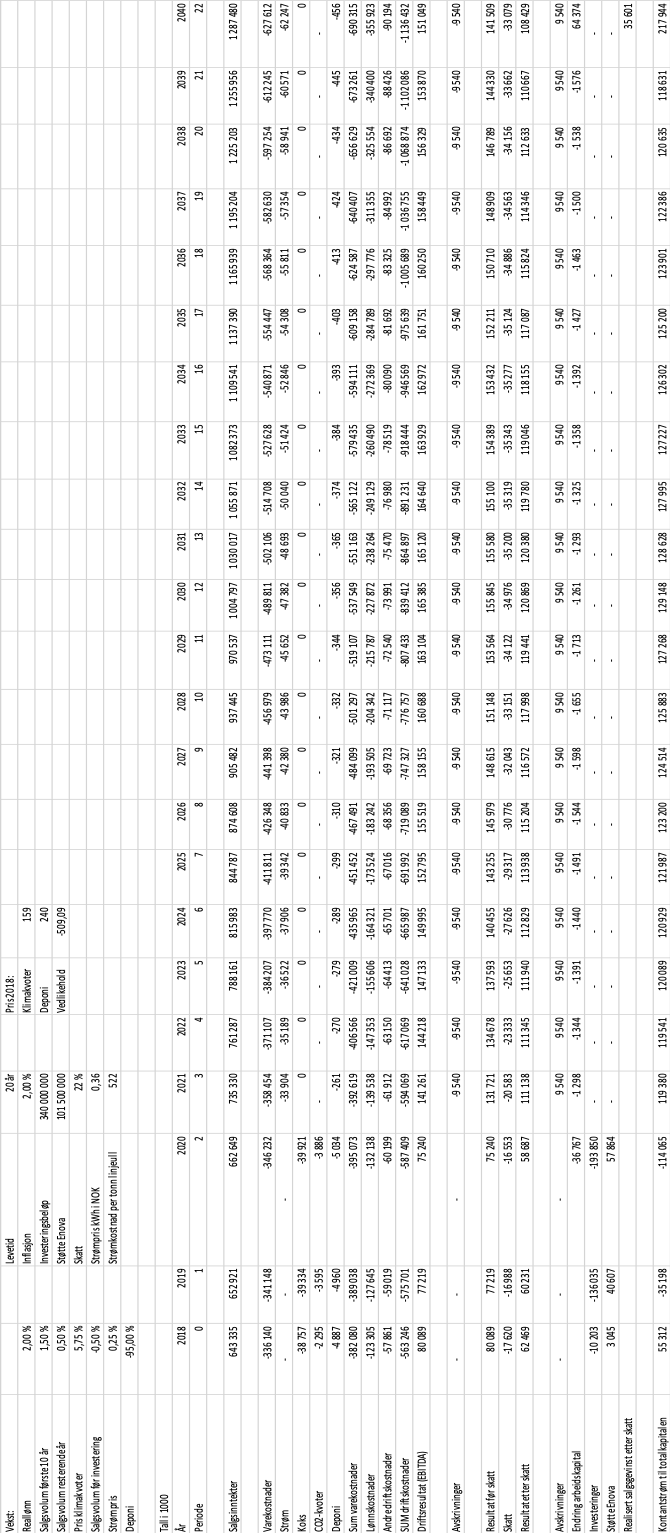
\includegraphics [scale=0.6]{appendiks/bilder/NNVelOvn.png}
\caption{Rockwool kontantstrøm ved ny el-ovn}
\label{fig:NNVelOvn}
\end{figure}

\begin{figure}[H]
\centering
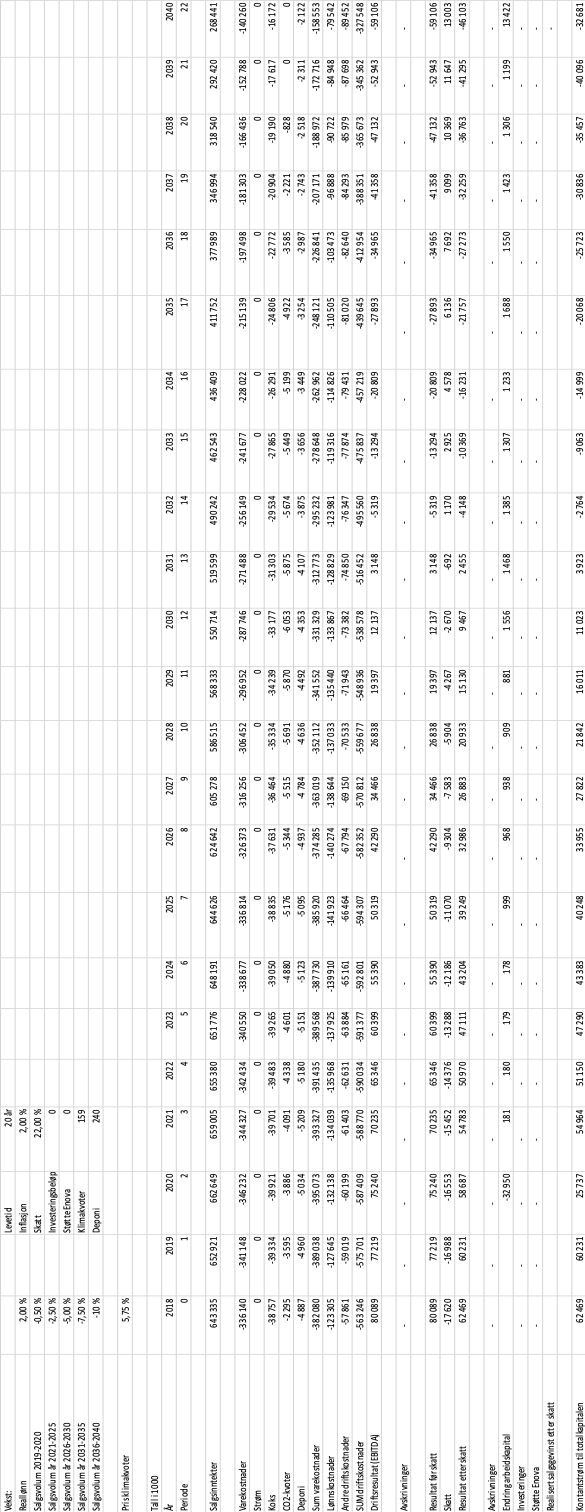
\includegraphics [scale=0.9]{appendiks/bilder/NNVnow.png}
\caption{Rockwool kontantstrøm ved nåværende løsning}
\label{fig:NNVnow}
\end{figure}

\begin{figure}[H]
\centering
\includegraphics [scale=0.8]{appendiks/bilder/NNVdiff.png}
\caption{Rockwool kontantstrøm differanse}
\label{fig:NNVdiff}
\end{figure}

\chapter{Logg}

\section*{11. Januar: Bachelor seminar}
Hele gruppen møter til første seminar som gjelder praktisk info om oppgaveskriving. Vi er i gang. 

\section*{25. Februar: Etablerer kontakt med AS Rockwool}
Kom i kontakt med fabrikksjef Erik Ølstad i Rockwool’s avdeling i Moss. Kommer frem til en mulig problemstilling som gjelder virksomhetens nylige beslutning om å investere i ny elektrisk smelteovn. Sender mail til Espen denne kvelden for å få godkjent problemstillingen.

\section*{26. Februar: Mailkorrespondanse }
Får positivt signal fra Espen vedrørende problemstilling. Oppgaven er i gang.

\section*{1. Mars: Fremføring og veiledning}
Gruppen presenterer problemstillingen og mulige fremgangsmåter foran Espen og medelever. Ettersom vi er helt i startfasen benytter vi også muligheten til en veiledningstime. Espen belyser viktige momenter for oppgaveløsning.

\section*{24. April: Møte med Erik Ølstad:}
Møter fabrikksjef Erik Ølstad for å få svar og oppklaring i spørsmål som har dukket opp underveis. 

\section*{12. Mai: Besøker fabrikken i Moss}
Erik Ølstad guider oss gjennom fabrikken i Moss. Viser oss plantegning for den nye el-ovnen. Vi benytter også muligheten til å stille spørsmål om ting vi ønsker belyst. 

\section*{22. Mai: “Drop-in” veiledning} 
Etter å ha møtt på flere utfordringer møter ett av gruppemedlemmene på kontordøra til Espen. Espen tar seg tid til en kort veiledning og sentrale spørsmål rundt oppgaveløsningen blir belyst. 

\section*{3. Juni: Innlevering}
Tre år på Handelshøyskolen BI er historie i det vi leverer Bacheloroppgaven. Takk for oss!  

\end{document}
